\PassOptionsToPackage{unicode}{hyperref}
\PassOptionsToPackage{hyphens}{url}
%
\documentclass[
  11pt,
  answers  
]{exam}
\usepackage[fleqn]{amsmath}
\usepackage[]{plex-otf}
\usepackage{iftex}
\usepackage[a4paper, margin=2.5cm]{geometry}
\usepackage{graphicx}
% \ifPDFTeX
%   \usepackage[T1]{fontenc}
%   \usepackage[utf8]{inputenc}
%   \usepackage{textcomp} % provide euro and other symbols
% \else % if luatex or xetex
%   \usepackage{unicode-math}
%   \defaultfontfeatures{Scale=MatchLowercase}
%   \defaultfontfeatures[\rmfamily]{Ligatures=TeX,Scale=1}
% \fi
% Use upquote if available, for straight quotes in verbatim environments
\IfFileExists{upquote.sty}{\usepackage{upquote}}{}
\IfFileExists{microtype.sty}{% use microtype if available
  \usepackage[]{microtype}
  \UseMicrotypeSet[protrusion]{basicmath} % disable protrusion for tt fonts
}{}
\makeatletter
\makeatother
\usepackage{xcolor}
\IfFileExists{xurl.sty}{\usepackage{xurl}}{} % add URL line breaks if available
\IfFileExists{bookmark.sty}{\usepackage{bookmark}}{\usepackage{hyperref}}
\urlstyle{same} % disable monospaced font for URLs
\setlength{\emergencystretch}{3em} % prevent overfull lines
\providecommand{\tightlist}{%
  \setlength{\itemsep}{0pt}\setlength{\parskip}{0pt}}
\setcounter{secnumdepth}{-\maxdimen} % remove section numbering
\newlength{\cslhangindent}
\setlength{\cslhangindent}{1.5em}
\newlength{\csllabelwidth}
\setlength{\csllabelwidth}{3em}
\newlength{\cslentryspacingunit} % times entry-spacing
\setlength{\cslentryspacingunit}{\parskip}
\newenvironment{CSLReferences}[2] % #1 hanging-ident, #2 entry spacing
 {% don't indent paragraphs
  \setlength{\parindent}{0pt}
  % turn on hanging indent if param 1 is 1
  \ifodd #1
  \let\oldpar\par
  \def\par{\hangindent=\cslhangindent\oldpar}
  \fi
  % set entry spacing
  \setlength{\parskip}{#2\cslentryspacingunit}
 }%
 {}
\usepackage{calc}
\newcommand{\CSLBlock}[1]{#1\hfill\break}
\newcommand{\CSLLeftMargin}[1]{\parbox[t]{\csllabelwidth}{#1}}
\newcommand{\CSLRightInline}[1]{\parbox[t]{\linewidth - \csllabelwidth}{#1}\break}
\newcommand{\CSLIndent}[1]{\hspace{\cslhangindent}#1}
\ifLuaTeX
  \usepackage{selnolig}  % disable illegal ligatures
\fi
\renewcommand{\solutiontitle}{\noindent\textbf{Jawab:}\par\noindent}
\newcommand{\mytitle}{Programming Fundamentals (IF 130)}
\newcommand{\theauthor}{Rivo Juicer Wowor}
\newcommand{\affiliation}{00000059635}

% \title{\textbf{\mytitle}}
% \author{\theauthor \
		% \small{\affiliation}}
% \date{}

% \usepackage{fancyhdr}
\lhead{\footnotesize{\textbf{\mytitle}}}%
\rfoot{\thepage}%
\cfoot{}
\lfoot{\footnotesize{\theauthor \hspace{1pt} (\affiliation)}}
\pagestyle{headandfoot}

% \pagestyle{plain}
\setlength{\parindent}{2em}
\renewcommand{\baselinestretch}{1.5}
\hbadness=99999
\usepackage{enumitem}
\unframedsolutions

\usepackage{graphicx}
\usepackage{listings}
\lstdefinestyle{mystyle}{
	showtabs=false,                  
  tabsize=3,
	basicstyle=\linespread{0.6},
  breaklines=true,
  postbreak=\mbox{\textcolor{red}{$\hookrightarrow$}\space},
  keywordstyle=\color{black}\bfseries,
  keywords={ ,BEGIN, START, END, DECLARE, SET, PROMPT, GET, PRINT, IF, ENDIF, WHILE, ENDWHILE, DO, UNTIL, FOR, CASE, ENDCASE, ENDFOR, Display, NOT, &&, ||, },
}
\lstset{style=mystyle}

\begin{document}
	\begin{titlepage}
		\centering
		\vspace{2cm}
		
\includegraphics[width=0.5\textwidth]{../../ref/logoUMN.png}\par\vspace{1cm}
		\vspace{1.5cm}
		\Large{Midterm Assignment} \par
		\vspace{1cm}
		\huge{\textbf{\mytitle}} \par
		\vspace{1.5cm}
		\Large{\theauthor} \par
		\emph{\affiliation} \par
		\vfill
		\today
	\end{titlepage}	

  \begin{questions}
    \question 
    % Buatlah algoritma dalam bentuk \textbf{flowchart modular} yang menerima 10 input angka dari pengguna, kemudian program akan menghitung jumlah dan total angka bilangan genap serta jumlah dari total angka bilangan ganjil.

    \begin{solution}
      \begin{center}
        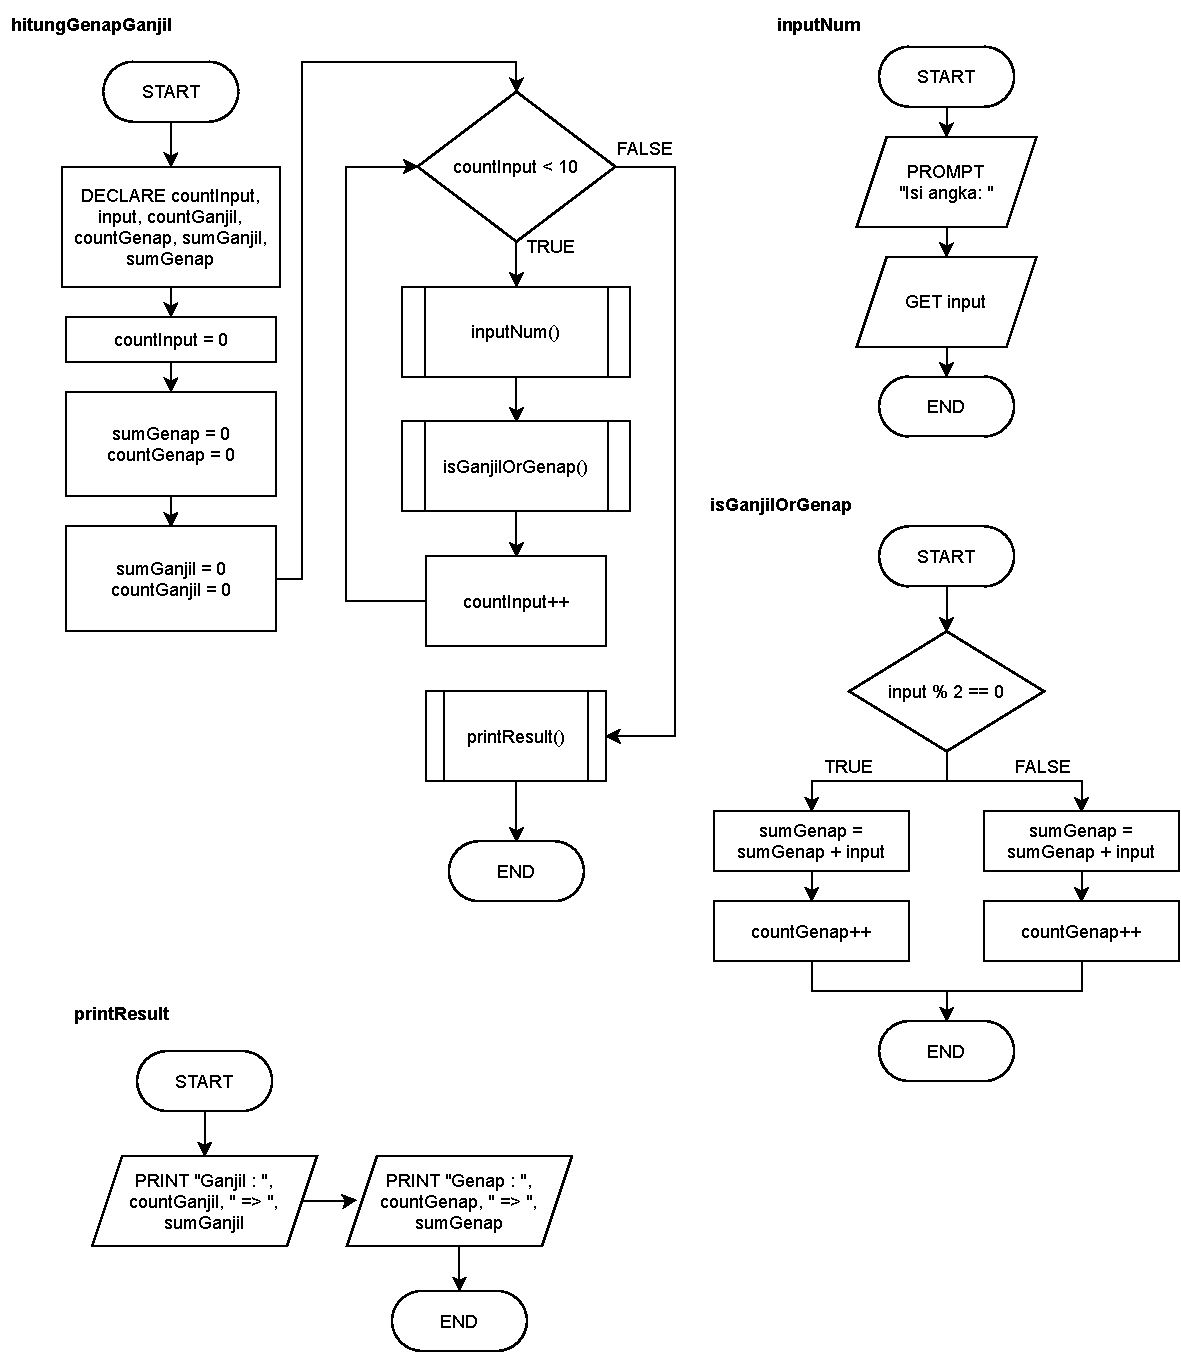
\includegraphics[clip, scale=0.8]{pdf/nomor1.pdf}
      \end{center}
    \end{solution}

    \pagebreak

    \question
    % Lakukan \textbf{desk checking} untuk \textbf{pseudocode} berikut dengan nilai \textbf{$in = 6$}. Tuliskan juga tampilan yang dihasilkan pada layar display!
    % \begin{lstlisting}
% Pseudocode_aneh
% 1  Prompt in
% 2  Get in
% 3  i = in
  %  WHILE (i >= 1)
% 4    j = 1
      %  DO
% 5        Display i
% 6        j = j + 1
      %  UNTIL (j>=i)
% 7      Display " "
% 8      i = i - 1
  %  ENDWHILE
% END
    % \end{lstlisting}
    % \pagebreak
    \begin{solution}
      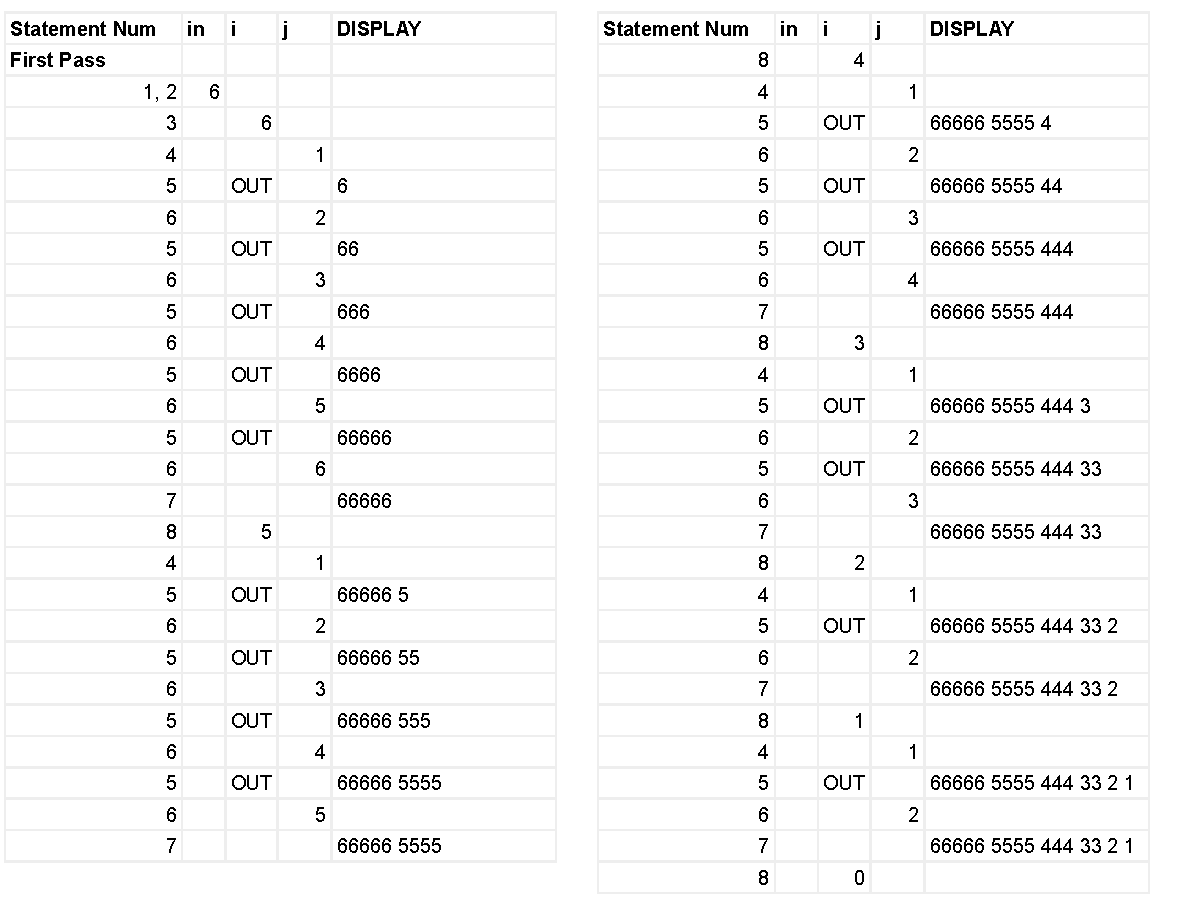
\includegraphics[clip, scale=0.85]{pdf/nomor2.pdf}
    \end{solution}
    \pagebreak
    
    \question
    Buatlah \textbf{modular pseudocode dengan passing parameter} untuk problem berikut. 
    Anda diminta untuk memasukkan sebuah bilangan positif n, dimana 1 n 15. Lakukan validasi input n tersebut dalam modul \textbf{inputn}.
    Jika nilai $n$ salah, maka akan mencetak pesan \emph{"Salah"} dan proses memasukkan sebuah bilangan akan \textbf{diulang} kembali \textbf{sampai benar}.
    Sebaliknya, jika nilai $n$ benar, maka akan memanggil modul \textbf{cetak} untuk mencetak tampilan segitiga berdasarkan nilai $n$ seperti pada contoh.

    \begin{solution}
      \begin{lstlisting}
main()
BEGIN
	DECLARE input
	input = input_n()
	cetak(input)
END	

input_n()
BEGIN
	DECLARE angkaValid, input
	DO
		PROMPT "Isi angka: "
		GET input
		IF NOT (input >= 1 && input <= 15) 
			PRINT "Salah"
			angkaValid == FALSE
		ELSE
			angkaValid == TRUE
		ENDIF
	WHILE (angkaValid == TRUE)
	RETURN input
END
      \end{lstlisting}
      \pagebreak
      \begin{lstlisting}
cetak(n)	
BEGIN
	DECLARE counter
	counter = 1
	WHILE counter <= n
		IF (counter > 9)
			PRINT counter - 10
		ELSE
			PRINT counter
		ENDIF
	ENDWHILE
END
      \end{lstlisting}
    \end{solution}
    \pagebreak
    \question
    \begin{solution}
      \begin{lstlisting}
deretanAngka
BEGIN
	DECLARE input, min, max, avg, numCount
	min, max, avg = 0
	WHILE (input != 0)
		GET input
		numCount++
		IF (min > input || min == 0)
			min = input
		ENDIF
		IF (max < input || max == 0)
			max = input
		ENDIF
		avg = avg + input
	ENDWHILE
	avg = avg / numCount
	PRINT "minimum = ", min
	PRINT "maksimum = ", max
	PRINT "rata-rata = ", avg
	PRINT "Terima Kasih"
END
      \end{lstlisting}
      \pagebreak
      \textbf{Flowchart} \par
      \vspace{2cm}
      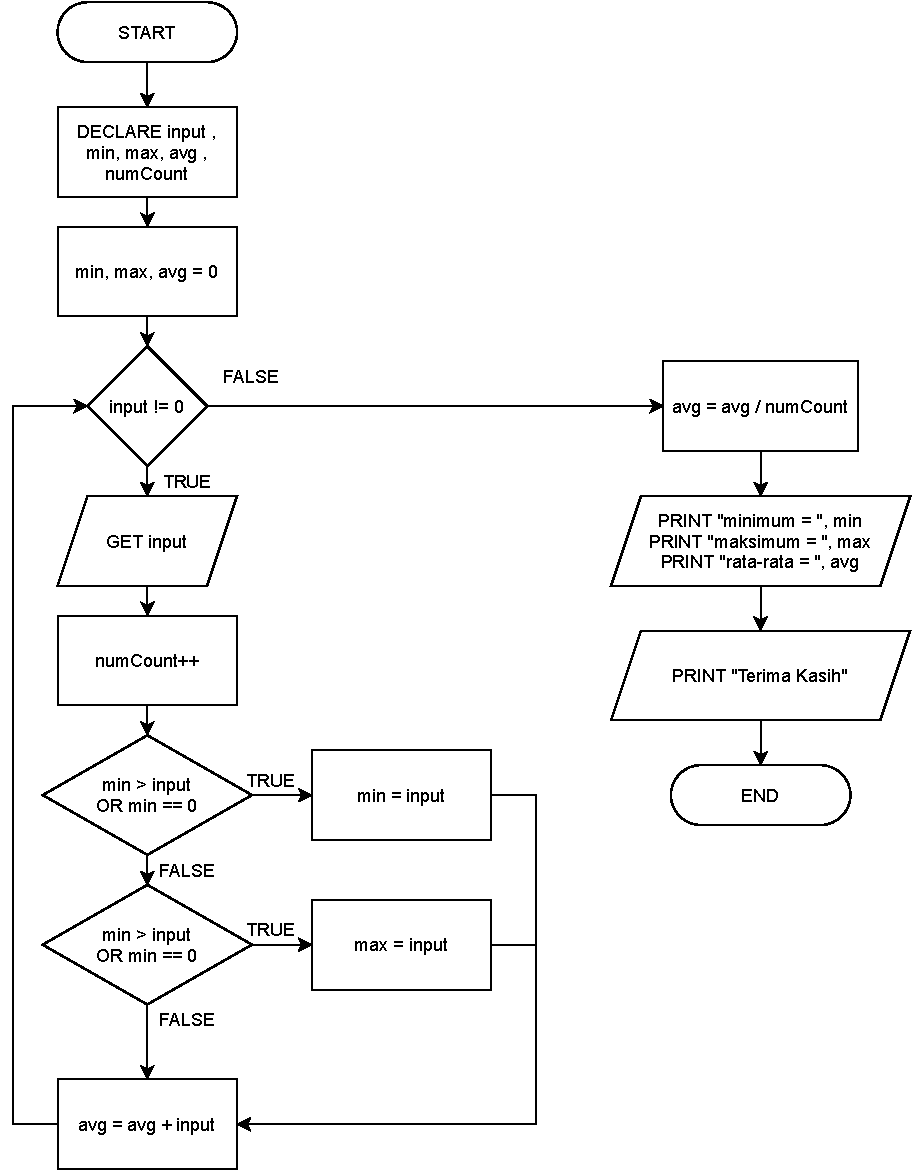
\includegraphics[clip,scale=0.8]{pdf/nomor3.pdf}
    \end{solution}
    \pagebreak
    \question
    \begin{solution}
      \begin{lstlisting}
timesUntilTen
BEGIN
	DECLARE result
	FOR (SET num1 = 1; num1 <= 10; num1++)
		FOR (SET num2 = 1; num2 <= 10; num2++)
			result = num1 * num2
			PRINT num1, " x ", num2, " = ", result
		ENDFOR
	ENDFOR
END
      \end{lstlisting}
    \end{solution}
  \end{questions}
\end{document}
